\section{Metric spaces}\label{sec:metric_spaces}

\begin{definition}\label{def:metric_space}\cite[248]{Engelking1989}
  A \ul{metric space} is a set $X$ along with a function $\mu: X \times X \to \BB{R}^{\geq 0}$, called a \ul{metric} or \ul{distance function}, such that
  \begin{description}
    \DItem{identity}{def:metric_space/identity} $\mu(x, y) = 0 \iff x = y$
    \DItem{symmetry}{def:metric_space/symmetry} $\mu(x, y) = \mu(y, x)$
    \DItem{triangle inequality}{def:metric_space/triangle_inequality} $\mu(x, y) \leq \mu(x, z) + \mu(z, y)$
  \end{description}

  If instead of \ref{def:metric_space/identity} we have the weaker condition
  \begin{description}
    \DItem{pseudometric identity}{def:metric_space/pseudometric_identity} $\forall x \in X, \mu(x, x) = 0$,
  \end{description}
  we call $\mu$ a \ul{pseudometric} and $(X, \mu)$ a \ul{pseudometric space}.

  \begin{defenum}
    \item\label{def:metric_space/subspace} If $A \subseteq X$ is a set, then $(A, \mu{\restriction_A})$ is a metric space and is called a \ul{subspace}.

    \item\label{def:metric_space/ball} Define the function
    \begin{align*}
      &B: X \times \BB{R}^{>0} \to \Power(X), \\
      &B(x, r) \coloneqq \{ y \in X \colon \mu(x, y) = r \}.
    \end{align*}

    The set $B(x, r)$ is called a \ul{ball with center $x$ and radius $r$}.

    \item\label{def:metric_space/closed_ball} The set
    \begin{align*}
      \Ol{B(x, r)} \coloneqq \Cl(B(x, r))
    \end{align*}
    is called the \ul{closed ball with center $x$ and radius $r$}.

    \item\label{def:metric_space/closed_ball} The set
    \begin{align*}
      S(x, r) \coloneqq \partial{B(x, r)}
    \end{align*}
    is called the \ul{sphere with center $x$ and radius $r$}.

    \item\label{def:metric_space/bounded_set} A set $A \subseteq X$ is called \ul{bounded} if it is contained in some ball $B(x, r)$.

    \item\label{def:metric_space/bounded_metric} If every set is bounded, we say that the metric itself is bounded.

    \item\label{def:metric_space/diameter} Define the function
    \begin{align*}
      &\Diam: \Power(X) \to \BB{R}^{\geq 0}, \\
      &\Diam(A) \coloneqq \sup \{ \mu(x, y) \colon x, y \in A \}.
    \end{align*}

    We call the number $\Diam(A)$ the \ul{diameter of $A$}.

    \item\label{def:metric_space/distance} Define the function
    \begin{align*}
      &\Dist: X \times \Power(X) \to \BB{R}^{\geq 0}, \\
      &\Dist(x, A) \coloneqq \inf \{ \mu(x, a) \colon a \in A \}.
    \end{align*}

    We call the number $\Dist(x, A)$ the \ul{distance from the point $x$ to the set $A$}. We use the convention that the infimum of an empty set of real numbers is $+\infty$, hence $\Dist(x, \varnothing) = \infty$.
  \end{defenum}
\end{definition}

\begin{note}\label{note:bounded_set_metric_order_equivalence}
  A set $A$ in a metric space $(X, \mu)$ is bounded\Tinyref{def:metric_space/bounded_set} if and only if the set $\{ \mu(a, b) \colon a, b \in A \}$ is bounded as a poset\Tinyref{def:poset/bounded_set}.
\end{note}

\begin{definition}\label{def:metric_topology}\cite[249]{Engelking1989}
  Let $(X, \mu)$ be a metric space. We define the \ul{metric topology} or \ul{induced topology} $\Cal{T}$ as the topology\Tinyref{def:topological_space} generated by the neighborhood system\Tinyref{def:topological_local_base}
  \begin{align*}
    \Cal{B}(x) \coloneqq \{ B (x, r) \colon r \in \BB{R}^{>0} \}.
  \end{align*}

  If for some topological space $(X, \Cal{T})$ there exists a metric such that $\Cal{T}$ is its induced topology, we say that the topology $\Cal{T}$ is \ul{metrizable}.
\end{definition}
\begin{proof}
  This is indeed a neighborhood system as it satisfies \ref{thm:topological_local_base_axioms/BP1}-\ref{thm:topological_local_base_axioms/BP3}:

  \begin{description}
    \item[\ref{thm:topological_local_base_axioms/BP1}] Every point $x$ obviously belongs to any ball centered at $x$.

    \item[\ref{thm:topological_local_base_axioms/BP2}] Fix $x \in X$ and two balls $B(x, r)$ and $B(x, s)$. Then
    \begin{align*}
      B(x, \min\{ r, s \}) \subseteq B(x, r) \cap B(x, s).
    \end{align*}

    \item[\ref{thm:topological_local_base_axioms/BP3}] Fix $x, y \in X$ and let $x \in B(y, r)$, i.e. $\mu(x, y) < r$.

    Define
    \begin{align*}
      s \coloneqq \min\{ \mu(x, y), \frac 1 n - \mu(x, y) \}.
    \end{align*}

    Let $z \in B(x, s)$. There are two cases:
    \begin{itemize}
      \item if $\mu(x, y) \leq \tfrac r 2$, then
      \begin{align*}
        \mu(z, y)
        \leq
        \mu(z, x) + \mu(x, y)
        <
        s + \mu(x, y)
        \leq
        \mu(x, y) + \mu(x, y)
        \leq
        2 \tfrac r 2
        =
        r.
      \end{align*}

      \item if $\mu(x, y) > \tfrac r 2$, then
      \begin{align*}
        \mu(z, y)
        \leq
        \mu(z, x) + \mu(x, y)
        <
        s + \mu(x, y)
        \leq
        (r - \mu(x, y)) + \mu(x, y)
        =
        r.
      \end{align*}
    \end{itemize}

    In both cases, $B(x, s) \subseteq B(y, r)$.

    \begin{center}
      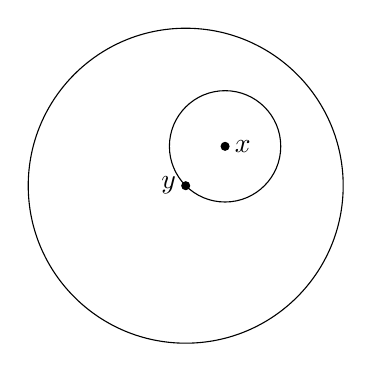
\begin{tikzpicture}
        \filldraw (0.5, 0.5) circle (0.05) node[right] {$x$};
        \draw (0.5, 0.5) circle (0.707);

        \filldraw (0, 0) circle (0.05) node[left] {$y$};
        \draw (0, 0) circle (2);
      \end{tikzpicture}
      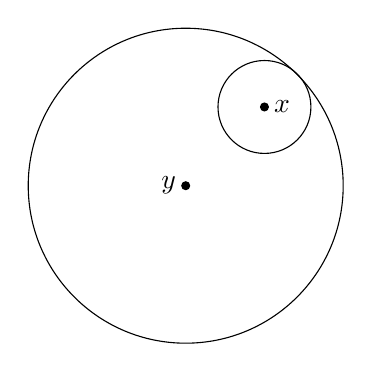
\begin{tikzpicture}
        \filldraw (1, 1) circle (0.05) node[right] {$x$};
        \draw (1, 1) circle (0.59);

        \filldraw (0, 0) circle (0.05) node[left] {$y$};
        \draw (0, 0) circle (2);
      \end{tikzpicture}
    \end{center}
  \end{description}
\end{proof}

\begin{proposition}\label{thm:locally_countable_metric_topology}
  The following is an alternative base for the metric topology\Tinyref{def:metric_topology}:

  \begin{align*}
    \Cal{B}(x) \coloneqq \{ B (x, \tfrac 1 n) \colon n = 1, 2, 3, \ldots \}.
  \end{align*}
\end{proposition}
\begin{proof}
  The proof is the same as in \cref{def:metric_topology}, except for a slight tweak in \ref{thm:topological_local_base_axioms/BP3}, where we define $m$ to be the the smallest positive integer such that
  \begin{align*}
    \tfrac 1 m \leq \min\{ \mu(x, y), r - \mu(x, y) \}.
  \end{align*}

  Note that $m$ exists by \cref{thm:ordinals_are_well_ordered}.

  We then obtain $B(x, \tfrac 1 m) \subseteq B(y, \tfrac 1 n)$.
\end{proof}

\begin{proposition}\label{thm:metric_topology_properties}
  The metric topology $\Cal{T}$ on $X$ induced by $\mu$ has the following properties:
  \begin{defenum}
    \item\label{thm:metric_topology_properties/ball_is_open} For every point $x \in X$ and any radius $r > 0$, the ball $B(x, r)$ is an open set and, hence, a neighborhood of $x$.
    \item\label{thm:metric_topology_properties/first_countable} $\Cal{T}$ is first-countable.
    \item\label{thm:metric_topology_properties/hausdorff} $\Cal{T}$ is Hausdorff.
  \end{defenum}
\end{proposition}
\begin{proof}
  \begin{description}
    \item[\ref{thm:metric_topology_properties/ball_is_open}] Obvious from \cref{def:metric_topology}.

    \item[\ref{thm:metric_topology_properties/first_countable}] Since \cref{thm:locally_countable_metric_topology} involves generating a topology using a neighborhood system of countable local neighborhoods, $\Cal{T}$ is first-countable.

    \item[\ref{thm:metric_topology_properties/hausdorff}] Let $x, y \in X$ be distinct points. Define
    \begin{align*}
      r \coloneqq \dfrac 1 2 \mu(x, y),
    \end{align*}
    so that
    \begin{align*}
      B(x, r) \cap B(y, r) = \varnothing.
    \end{align*}
  \end{description}
\end{proof}

\begin{proposition}\label{thm:metric_convergence_iff_metric_topology_convergence}
  Let $(X, \mu)$ be a metric space and $\Cal{T}$ be the induced metric topology\Tinyref{def:metric_topology}. The convergence\Tinyref{sec:convergence} in $\Cal{T}$ is the completely described by sequences, that is,

  \begin{defenum}
    \item\label{thm:metric_convergence_iff_metric_topology_convergence/hausdorff} every converging net\Tinyref{def:topological_net} has a single limit.

    \item\label{thm:metric_convergence_iff_metric_topology_convergence/cluster_point} $x \in X$ is a cluster point\Tinyref{def:net_cluster_point} of the sequence $\{ x_i \}_{i=1}^\infty$ if and only if for every positive real number $\varepsilon > 0$ and every index $i_0$ there exists an index $i_\varepsilon > i_0$ such that
    \begin{align*}
      \mu(x, x_{i_\varepsilon}) < \varepsilon.
    \end{align*}

    \item\label{thm:metric_convergence_iff_metric_topology_convergence/limit_point} $x \in X$ is a limit point\Tinyref{def:net_limit_point} of the sequence $\{ x_i \}_{i=1}^\infty$ if and only if for every positive real number $\varepsilon > 0$ there exists an index $i_0$ such that
    \begin{align*}
      i \geq i_0 \implies \mu(x, x_i) < \varepsilon.
    \end{align*}

    \item\label{thm:metric_convergence_iff_metric_topology_convergence/closure} given any set $A \subseteq X$, a point $x \in X$ belongs to $\Cl{A}$ if and only if there exists a sequence $\{ x_i \}_{i=1}^\infty \subseteq A$ such that $x_i \xrightarrow[i \to \infty]{} x$ (compare with \cref{thm:limit_point_iff_in_closure}).
  \end{defenum}
\end{proposition}
\begin{proof}
  \begin{description}
    \item[\ref{thm:metric_convergence_iff_metric_topology_convergence/single_limit}] Follows directly from \cref{thm:t2_iff_singleton_limits} and \cref{thm:metric_topology_properties/hausdorff}.

    \item[\ref{thm:metric_convergence_iff_metric_topology_convergence/cluster_point}] Fix a sequence $x_i \to x$.

    \Implies Fix a radius $\varepsilon > 0$ and an index $i_0$. Note that $B(x, \varepsilon)$ is a neighborhood of $x$ and hence by \cref{def:net_cluster_point} there exists an index $i_\varepsilon \geq i_0$ such that $x_{i_U} \in B(x, \varepsilon)$, which is the same as
    \begin{align*}
      \mu(x, x_{i_U}) < \varepsilon.
    \end{align*}

    \ImpliedBy Fix a neighborhood $U$ of $x$. Since the topology is generated by a local base of balls, then $U$ contains some ball $B(x, r)$. Thus there exists an index $i_0$, such that
    \begin{align*}
      \mu(x, x_{i_r}) < r,
    \end{align*}
    hence
    \begin{align*}
      x_{i_r} \in B(x, r) \subseteq U.
    \end{align*}

    \item[\ref{thm:metric_convergence_iff_metric_topology_convergence/limit_point}] Similar to \ref{thm:metric_convergence_iff_metric_topology_convergence/cluster_point}.

    \item[\ref{thm:metric_convergence_iff_metric_topology_convergence/closure}]
    \Implies Fix a nonempty set $A$ and $x \in \Cl A$. If $x \in A$, then the constant sequence with all members equal to $x$ converges to $A$.

    Assume that $x \not\in A$ and choose any sequence\AOC
    \begin{align*}
      x_i \in B(x, \tfrac 1 i) \setminus \{ x \}, i = 1, 2, \ldots.
    \end{align*}

    Fix $\varepsilon > 0$. By \cref{thm:ordinals_are_well_ordered} there exists a least positive integer $i_0$ such that $\tfrac 1 i_0 < \varepsilon$. It follows that $x_i \to x$ since
    \begin{align*}
      i \geq i_0 \implies \mu(x, x_i) \leq \mu(x, x_{i_0}) \leq \varepsilon.
    \end{align*}

    \ImpliedBy Obvious
  \end{description}
\end{proof}

\begin{definition}\label{def:isometry}\cite[253]{Engelking1989}
  Let $(X, \mu)$ and $(Y, \nu)$ be two metric spaces\Tinyref{def:metric_space}. We say that the function $f: X \to Y$ is a \ul{distance preserving map} or \ul{isometry} or \ul{isometric embedding} if
  \begin{align*}
    \forall x, y \in X, \mu(x, y) = \nu(f(x), f(y)).
  \end{align*}

  If $f$ is bijective, we say that $X$ and $Y$ are \ul{isometric}.
\end{definition}

\begin{proposition}\label{def:isometry_is_injective}
  An isometry\Tinyref{def:isometry} $f: (X, \mu) \to (Y, \nu)$ is always injective.
\end{proposition}
\begin{proof}
  If $f(x) = f(x')$, then by \ref{def:metric_space/identity}, $x = x'$.
\end{proof}

\begin{definition}\label{def:category_of_metric_spaces}
  The class\Tinyref{def:set_zfc} of all metric spaces forms the category\Tinyref{def:category} $\Bold{Met}$, where for every two metric spaces $X, Y \in \Bold{Met}$, the morphisms $\Bold{Met}(X, Y)$ are the isometries\Tinyref{def:isometry} from $X$ to $Y$ and composition is the usual function composition\Tinyref{def:function_composition}.

  The category is concrete\Tinyref{def:concrete_category} and locally small\Tinyref{def:category_cardinality}.
\end{definition}
